\chapter[Quantifying Characteristics of the FD PMT]{\centering Quantifying Characteristics of \\ the Fluorescence Detector \\ Photomuliplier Tube \\}\label{Ch:PMTCharacter}

Characterising the PMT at 600V and 900V
\begin{itemize}
\item Using the characteristics of the PMT at 900V as a baseline
\item Measure linearity
\item ND filters vs Two LED method
\item temperature effects
\end{itemize}

\section{Motivation}

- Start off with moonlight explanation
- Looking at effects of increased NSB on equipment
- What type of PMT used

The aim is to use the measurements done at 900V as the baseline of expected performance and then observe the repeated measurements at 600V. We have a good  understanding of the characteristics of the PMT operating at 900V due to this being the nominal voltage that the PMTS in the FD telescopes are run at.

The Fluorescence Detectors (FDs) use Photomultiplier Tube (PMT) as camera pixels within the telescopes to view the Extensive Air Showers. The PMTs are operated at a gain of 5 $\times$ 10$^4$ electrons per photo-electron. This gain relates to a High Voltage about 900V. The investigation into running the Fluorescence Detectors under moonlight has lead to the thinking of running the PMTs under decreased PMT gain. The PMT gain is expected to decreased by a factor of 10 to compensate. Therefore the PMT High Voltage would be dropped to about 600V.

I explore the characteristics at 600V as we are expecting to to reduce the PMT gain by a factor of 10 and this related to an approximate voltage drop to 600V. This may be an over estimate but we can be confident if the PMT voltage used is greater then 600V then the characteristics will be the same.

\section{PMT Linearity}

One of the main characteristics of a Photomultiplier Tube (PMT) of importance its region of linearity. A PMT linearity is where if the light intensity doubles the PMT signal response doubles as well. It is important to quantify this region to be confident that if the light intensity changes the PMT response correspond.

I investigated at two methods to measure the PMT linearity - using Neutral Density filters and the Two LED method.

\subsection{Neutral Density Filters}

The Neutral Density (ND) method involves employing filters to reduce the light intensity reaching the PMT cathode by a known amount. The filters were used singularly and in combination to get different Optical Transmission values. The filters are labelled with optical density which is different to optical depth. To convert optical density to optical transmission:
\begin{equation}
\mathrm{Optical \ Density} = - \mathrm{log}_{10}\left(\frac{\mathrm{Optical \ Transmission}}{100} \right)
\end{equation}
To get different optical transmission values, the filters can be stacked and the optical density values just add together (eg. if using two filters, one with ND 0.4 and ND 0.1 the total ND will be 0.5).

I repeated a study done by Privitera et. al. (1990) \textbf{ref.} on Auger PMTs. I wanted to use the result at an High Voltage value of 900V as my baseline then continue my study to observe the result at an High Voltage value of 600V.

Some of the disadvantages of using Neutral Density filters it that you are restricted to fixed units of optical transmission depending on which filters you have access too. Also you are relying on the fact that the optical density doesn't change over time and is not effected by handling and storage. There is also some uncertainty on the optical density value quoted.

\begin{figure}
\centering
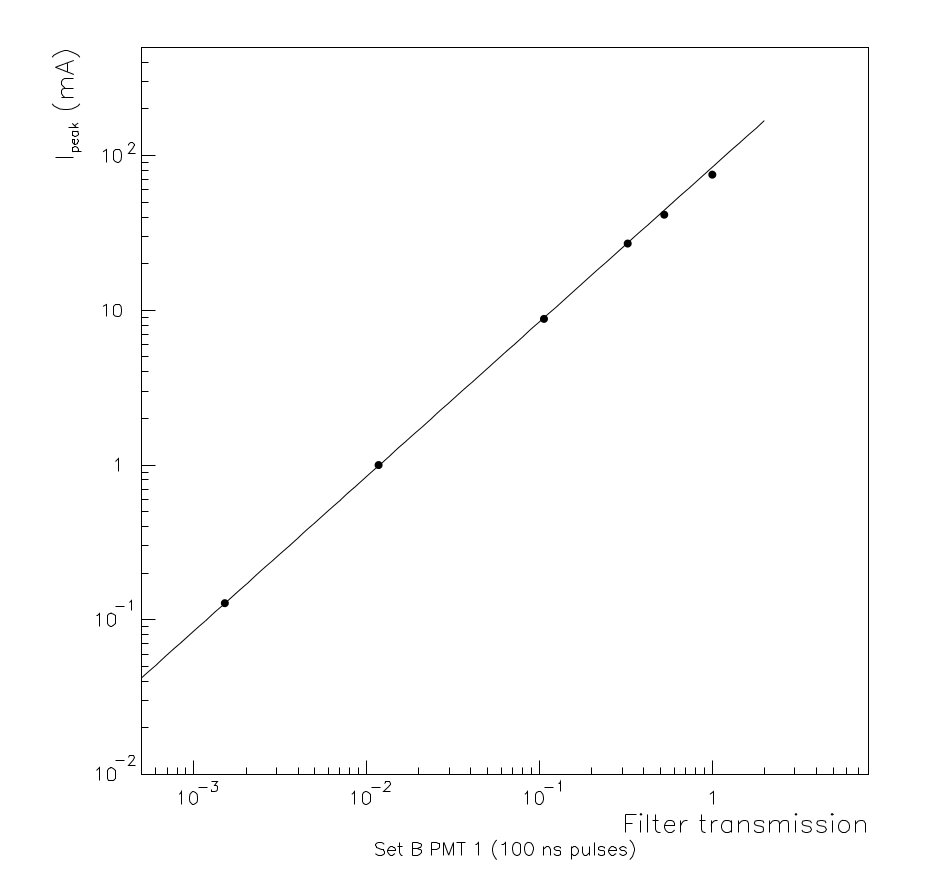
\includegraphics[width=\textwidth]{chapters/graphs/PMTchar/pmt_linearity_100V_privitera.png}
\caption{Previous PMT linearity test done by Privitera et. al. 1999 with Neutral density filters.}
\end{figure}

\begin{figure}
\centering
\begin{subfigure}[b]{\textwidth}
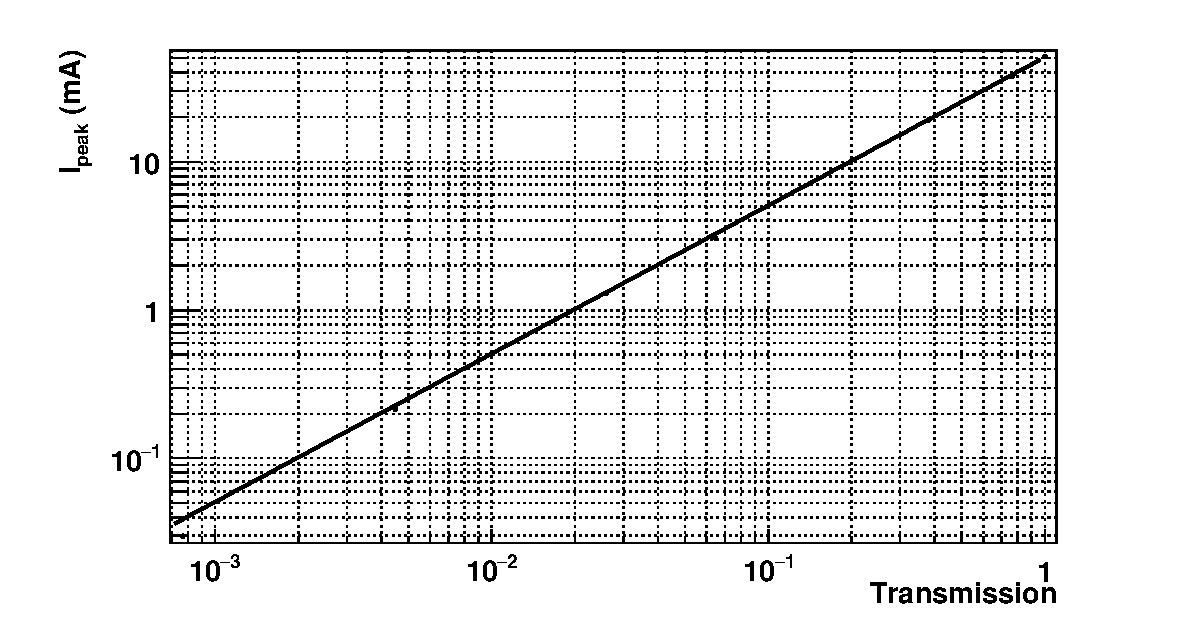
\includegraphics[width=\textwidth]{chapters/graphs/PMTchar/PMT900V_linearityNDmethod.pdf}
\caption{•}
\end{subfigure}
\begin{subfigure}[b]{\textwidth}
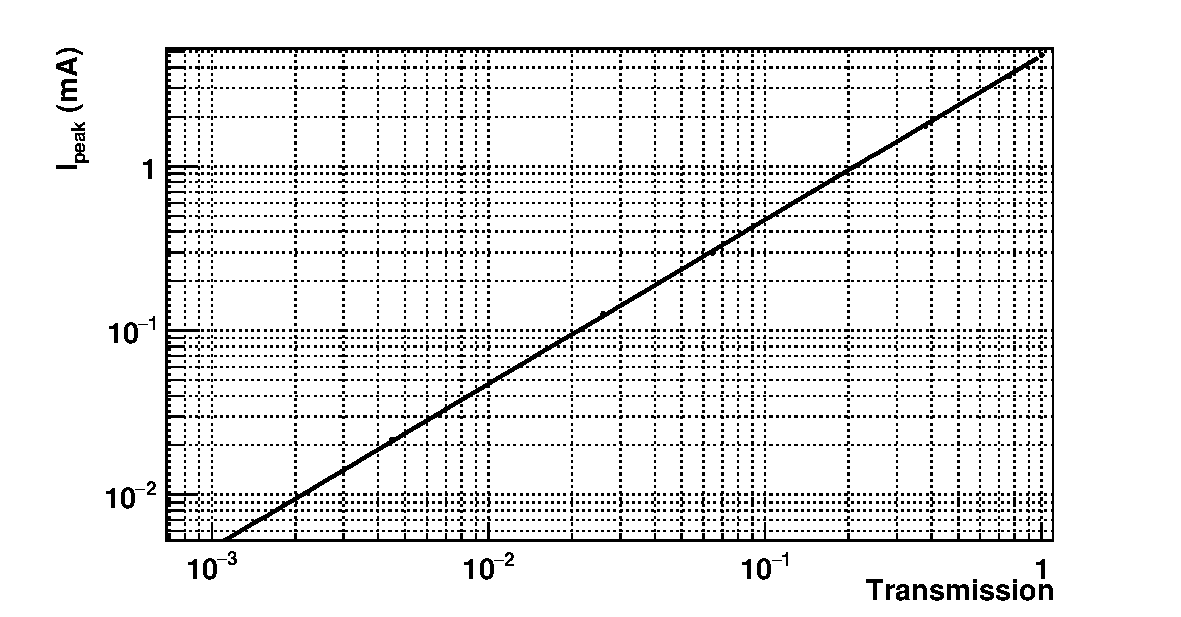
\includegraphics[width=\textwidth]{chapters/graphs/PMTchar/PMT600V_linearityNDmethod.pdf}
\caption{•}
\end{subfigure}
\caption{Neutral density method at 900V and 600V.}
\end{figure}

\subsection{Two LED Method}

Another method that was investigated was the two LED method. This method was first used in the original measurement of the SD PMTs \textbf{ref}. To measure the linearity, two LEDs are pointed at the PMT cathode and the first set of observation with the LEDs on separately. After one set taken with the LEDs on at the same time. A graphical representation is shown in Fig. \ref{fig:TwoLEDmethod_Setup} of the set-up used to measure the PMT linearity at both 900V and 600V. Two pulse generators are used to drive the LEDs separately and to allow the two pulses to overlap when needing to measure the PMT response to the LEDs on at the same time. To find the linearity a ratio is plotted against peak pulse ampere. The ratio is calculated with following the equation:
\begin{equation}
\mathrm{Ratio} = \frac{\mathrm{LED}_{1+2}}{\mathrm{LED}_{1} + \mathrm{LED}_{2}}
\end{equation}
Where LED$_{1+2}$ is the measurement of both LEDs are on at the same time, and LED$_{1}$ and LED$_2$ is the measurement when they are on separately. The principle employed here is that while the intensity is within the linearity region the peak of LED$_{1+2}$ should equal the addition of LED$_{1}$ and LED$_2$. \textbf{/* Possible repartition */} Therefore the ratio should be one while both peak anode ampere from the LEDs on individually and LEDs on together are within the region of linearity. As the light intensity is increased, the LEDs on together will move out of the region of linearity first. Typically this means that the peak ampere measured from both LEDs on at the same time will be less than the combination of the peak ampere when measured separately. This will cause the ratio to dip below one.

The advantages of this method is that any LED brightness can be used as long as the two LED intensities are different. With different LED brightnesses we were able to probe different region of linearity in the PMT. \textbf{Does this say anything?}

The result of the two LED Method is shown in Fig. \ref{fig:TwoLEDmethod_result} for both 900V and 600V. The x-axis is the peak ampere of the measured pulses when both LEDs are on at the same time. The plots show that while the peak anode currents change by a close factor of 10, the gain of the PMT has also been reduced by a similar factor. This seems to indicate that the cathode is the limiting factor for the linearity for this type of PMT. \textbf{Maybe quote theoretical peak anode current for a 10$^{21}$ eV shower}.

\begin{figure}
\centering
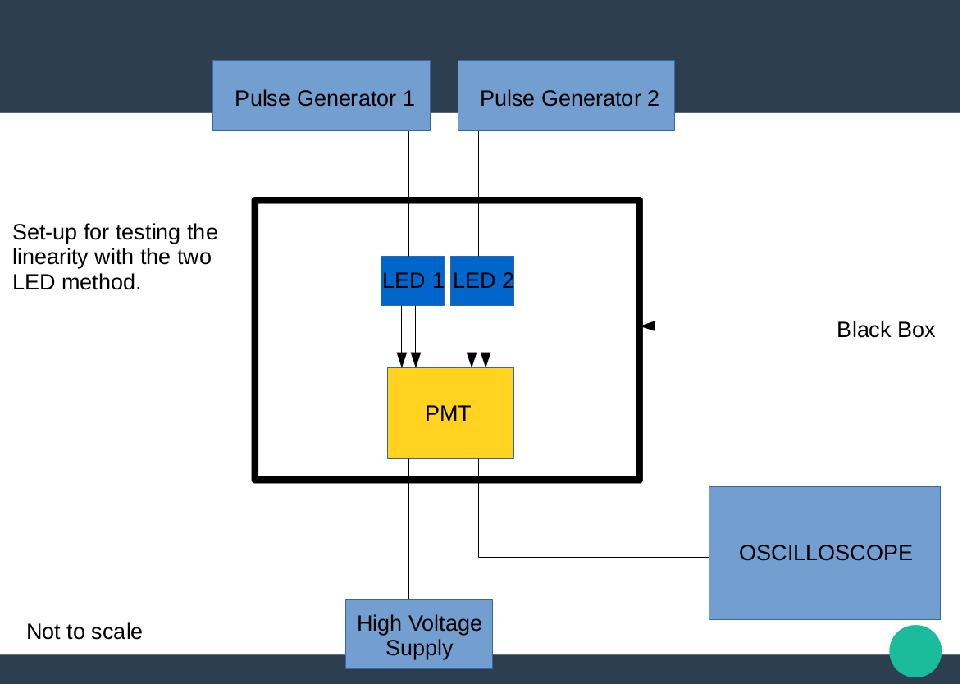
\includegraphics[width=\textwidth]{chapters/graphs/PMTchar/diagram_TwoLEDmethod.pdf}
\caption{A graphical respresention of the Two LED Setup used in the lab at University of Adelaide.}
\label{fig:TwoLEDmethod_Setup}
\end{figure}

\begin{figure}
\centering
\begin{subfigure}[b]{\textwidth}
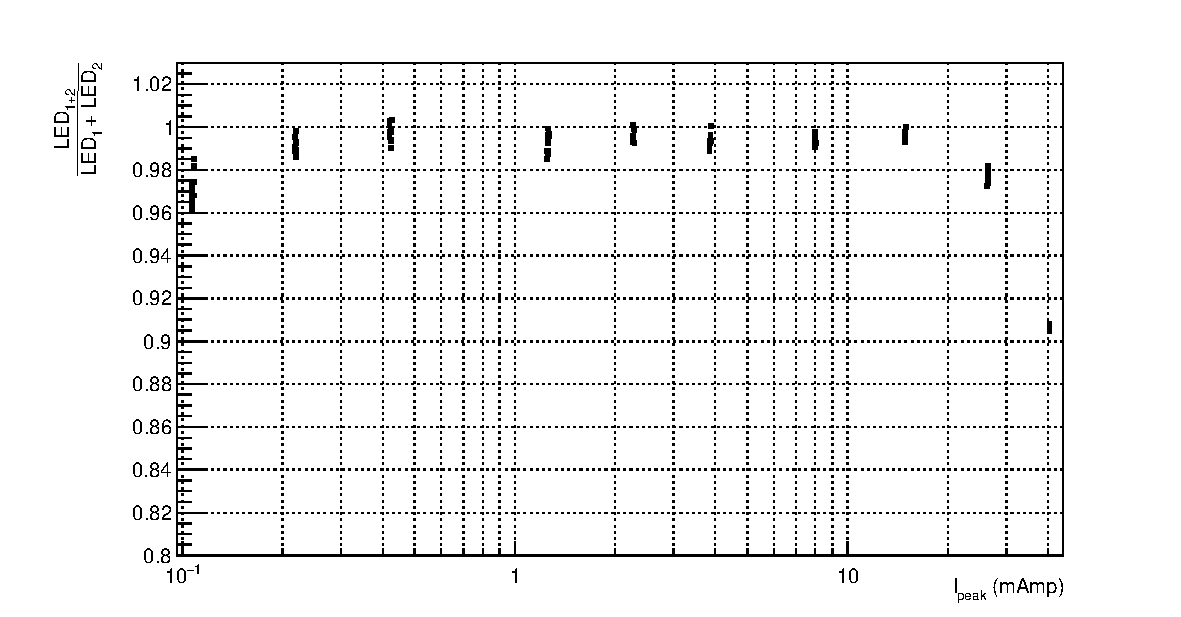
\includegraphics[width=\textwidth]{chapters/graphs/PMTchar/PMT900V_linearity2LEDmethod.pdf}
\caption{•}
\end{subfigure}
\begin{subfigure}[b]{\textwidth}
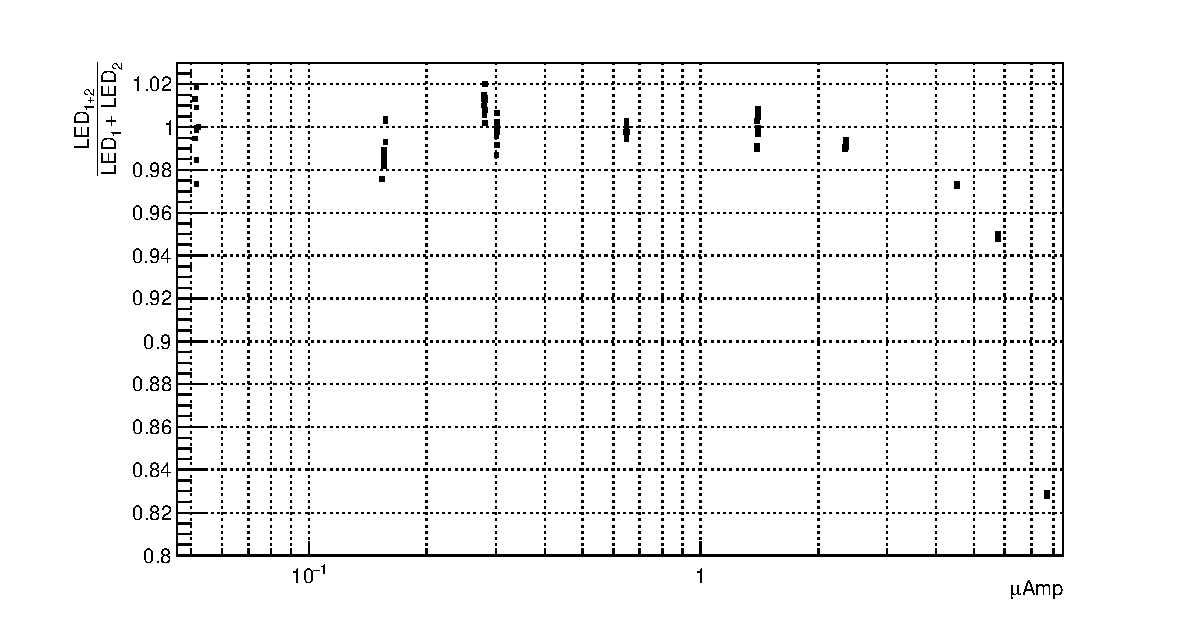
\includegraphics[width=\textwidth]{chapters/graphs/PMTchar/PMT600V_linearity2LEDmethod.pdf}
\caption{•}
\end{subfigure}
\caption{Two LED method at 900V and 600V.} \label{fig:TwoLEDmethod_result}
\end{figure}

\section{Effects of Temperature on PMT Gain}

Quoted on any PMT data sheet is the expected change in gain as a function of temperature. The XP3062 PMT used in the FD telescopes is quoted to be -0.2\%$\backslash$K. I measured this value in the lab at University of Adelaide at both 900V and 600V. The set-up to monitor the gain of the PMT involved a LED inside a copper oven pointed at the cathode which is pulsed once per second, and a temperature gauge. I was able to control the temperature inside the laboratory to see the gain change over a variety of temperature values. The LED was inside the copper oven to maintain an independent constant temperature so the number of photons emitted could considered to be fixed. The PMT was inside a box that highly light proof - the top was held down with screws, then two layers of black electrical tape was applied to the lid joinings and then a black out curtain was draped over the top. Only the temperature was allowed to vary over the measurement period. Therefore any changes in the absolute ADC measurements are related to changes in the PMT gain.

Measurements for temperature vs PMT gain was taken at both High Voltage values of 900V and 600V.The plots in Fig. \ref{fig:PMTtemp_v_gain} the effects of temperature on the PMT can be clearly seen at both high voltage values. For either high voltage value the measured PMT gain changer per K was -0.6\%$\backslash$K \textbf{needs uncertainty}. This maybe different to the quoted data sheet but is not unreasonable. The quoted data sheet is an average of many PMTs while this is a measurement of one particular PMT. What was interested was that this value did not deviate if using the PMT at 900V or 600V.


\begin{figure}
\centering
\begin{subfigure}[b]{\textwidth}
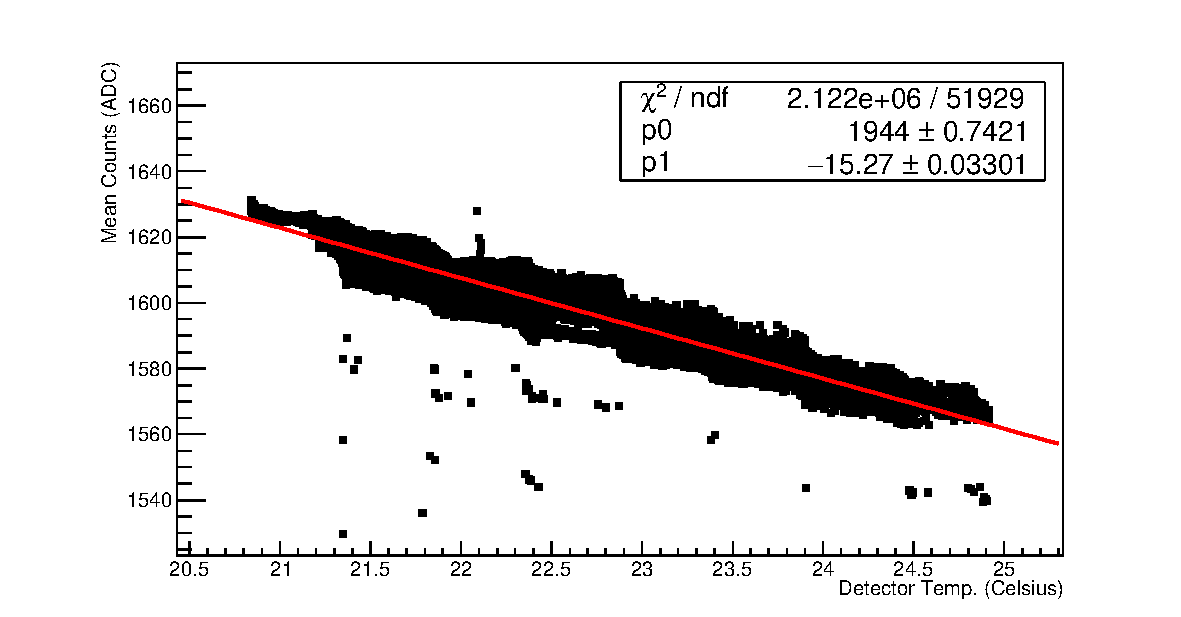
\includegraphics[width=\textwidth]{chapters/graphs/PMTchar/PMT900V_temperatureVsADC.pdf}
\caption{•}
\end{subfigure}
\begin{subfigure}[b]{\textwidth}
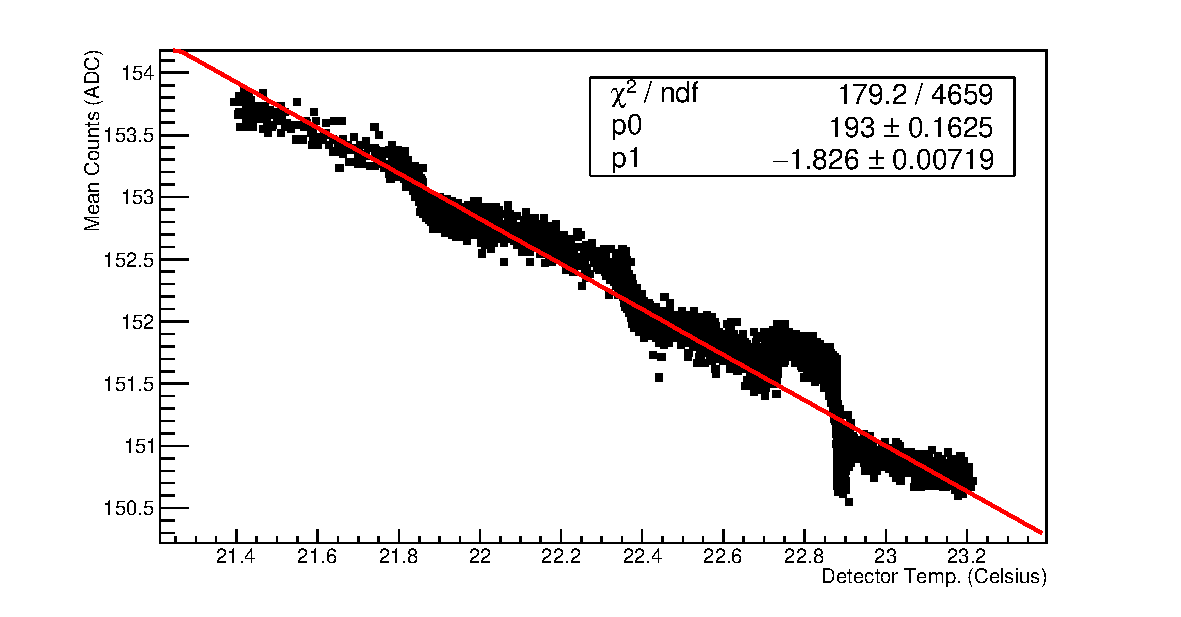
\includegraphics[width=\textwidth]{chapters/graphs/PMTchar/PMT600V_temperatureVsADC.pdf}
\caption{•}
\end{subfigure}
\caption{Showing the how PMT gain correlates with surrounding temperature.} \label{fig:PMTtemp_v_gain}
\end{figure}

